\documentclass{ctexart}
\usepackage{geometry}
\usepackage{endnotes}
\usepackage{graphicx}
\geometry{left=2cm,right=2cm,top=2.5cm,bottom=2.5cm}
\newtheorem{zhuanlan}{专栏}

\title{\textbf{人类减贫的中国实践}}
\author{中华人民共和国国务院新闻办公室}
\date{(2021年4月)}

\newcommand\sect[1]{\section*{#1}\addcontentsline{toc}{section}{#1}}
\renewcommand{\notesname}{注释}

\begin{document}

\maketitle

\tableofcontents

\sect{前言}

贫困是人类社会的顽疾,是全世界面临的共同挑战。贫困及其伴生的饥饿、疾病、社会冲突等一系列难题,严重阻碍人类对美好生活的追求。消除贫困是人类梦寐以求的理想,人类发展史就是与贫困不懈斗争的历史。

中国是拥有14亿人口、世界上最大的发展中国家,基础差、底子薄,发展不平衡,长期饱受贫困问题困扰。中国的贫困规模之大、贫困分布之广、贫困程度之深世所罕见,贫困治理难度超乎想象。

今年是中国共产党成立100周年。100年来,中国共产党团结带领人民,以坚定不移、顽强不屈的信念和意志与贫困作斗争。中共十八大以来,在以习近平同志为核心的党中央领导下,中国组织实施了人类历史上规模空前、力度最大、惠及人口最多的脱贫攻坚战。2021年2月25日,习近平总书记在全国脱贫攻坚总结表彰大会上庄严宣告,脱贫攻坚战取得了全面胜利,中国完成了消除绝对贫困的艰巨任务。

占世界人口近五分之一的中国全面消除绝对贫困,提前10年实现《联合国2030年可持续发展议程》减贫目标,不仅是中华民族发展史上具有里程碑意义的大事件,也是人类减贫史乃至人类发展史上的大事件,为全球减贫事业发展和人类发展进步作出了重大贡献。

贫穷不是命中注定,贫困并非不可战胜。中国减贫的实践表明,与贫困作斗争,最重要的是勇气、远见、责任和担当。只要有坚定意志和决心并付诸实际行动,就能够向着摆脱贫困、实现共同富裕的美好前景不断迈进。

为记录中国消除绝对贫困的伟大历程,介绍人类减贫的中国探索和实践,分享中国扶贫脱贫的经验做法,特发布本白皮书。

\section{中国共产党的庄严承诺}

中华民族是历史悠久、勤劳智慧的民族,创造了辉煌灿烂的中华文明。中华民族又是饱经苦难的民族,广大劳动人民长期处于贫困状态。几千年来,中国人民始终为摆脱贫困艰难求索。近代以后,在封建腐朽统治和西方列强侵略下,中国沦为半殖民地半封建社会,亿万民众处于贫困甚至赤贫状态。中国人民始终不屈不挠、奋力抗争,始终梦想实现国家富强、民族复兴,始终梦想过上幸福美好的生活。

\subsection{中国共产党领导人民夺取革命胜利,建立新中国,开启了实现国家富强、人民富裕的崭新历程}

1921年7月,中国共产党诞生。中国产生了共产党,这是开天辟地的大事变。从诞生之日起,中国共产党就把为中国人民谋幸福、为中华民族谋复兴作为初心使命,团结带领人民为创造自己的美好生活进行了长期艰辛奋斗。以毛泽东同志为核心的第一代中央领导集体,把农民翻身解放作为革命的基本问题,领导人民进行土地革命、实行“耕者有其田”,推翻了帝国主义、封建主义和官僚资本主义的反动统治,取得新民主主义革命胜利,建立了新中国,结束了中国人民长期以来遭受压迫与剥削的历史,结束了国家战乱频仍、四分五裂的局面,实现了民族独立和人民解放,为中国摆脱贫穷落后、实现繁荣富强扫清了障碍、创造了根本政治条件。

1949年10月1日,中华人民共和国成立,中国人民从此站立起来、当家做主,真正成为新国家新社会的主人。面对一穷二白、百业凋敝的困难局面,中国共产党团结带领人民自力更生、艰苦奋斗,发奋图强、重整山河。在全国开展轰轰烈烈的土地改革,延续2000多年的封建土地制度被废除,消除了造成农民贫困的主要制度因素。对农业、手工业和资本主义工商业进行社会主义改造,建立起社会主义基本制度,为从根本上解决贫困问题提供了最基本制度保证。开展大规模社会主义建设,建立独立的、比较完整的工业体系和国民经济体系,大力发展集体经济,大兴农田水利。大办农村教育和合作医疗,探索建立以集体经济为基础、以“五保”制度\endnote{《1956年到1967年全国农业发展纲要》明确提出,农业合作社对于社内缺乏劳动力、生活没有依靠的鳏寡孤独的社员,在生活上给予适当照顾,做到保吃、保穿、保烧(燃料)、保教(儿童和少年)、保葬,使他们的生养死葬都有指靠。}和特困群体救济为主体的农村初级社会保障体系。社会主义建设在曲折中向前推进,人民物质生活和文化水平逐步提高,占世界近四分之一人口的中国人民特别是农民的基本生活需求得到初步满足。

\subsection{改革开放极大促进了中国发展,中国减贫进程加快推进}

1978年12月,中共中央召开十一届三中全会,开启了中国改革开放和社会主义现代化建设新时期。改革开放是中国人民和中华民族发展史上的又一次伟大革命,为中国注入了创新和发展的强大动力。中国经济社会快速发展,中国减贫进程加快推进,贫困人口大幅度减少。

改革开放初期,面对中国农村贫困人口基数大、贫困发生率高的严峻形势,以邓小平同志为核心的第二代中央领导集体,作出“贫穷不是社会主义,社会主义要消灭贫穷”的重要论断,提出到20世纪末人民生活达到小康水平的目标,制定“三步走”发展战略\endnote{中共十三大提出,党的十一届三中全会以后,中国经济建设的战略部署大体分三步走。第一步,实现国民生产总值比1980年翻一番,解决人民的温饱问题。第二步,到20世纪末,使国民生产总值再增长一倍,人民生活达到小康水平。第三步,到21世纪中叶,人均国民生产总值达到中等发达国家水平,人民生活比较富裕,基本实现现代化。},提出“两个大局”的战略构想\endnote{1988年,邓小平同志明确提出:“沿海地区要加快对外开放,使这个拥有两亿人口的广大地带较快地先发展起来,从而带动内地更好地发展,这是一个事关大局的问题。内地要顾全这个大局。反过来,发展到一定的时候,又要求沿海拿出更多力量来帮助内地发展,这也是个大局。那时沿海也要服从这个大局。”来源:《邓小平文选》第三卷。},实施一系列农业农村重大改革,从国家层面开展大规模、有计划、有组织的扶贫开发。在农村实施以家庭联产承包为主的生产责任制和统分结合的双层经营体制,理顺了农村最基本的生产关系,调动了农民生产积极性,使农业生产迅速扭转了长期徘徊不前的局面。实施农产品流通体制改革,大力发展乡镇企业,促进了农村整体收入水平提高。成立专门扶贫机构,确定了扶贫标准、重点片区和贫困县,启动实施“三西”\endnote{“三西”指甘肃省河西地区、定西地区和宁夏回族自治区西海固地区,是改革开放初期全国集中连片最困难的地区之一。1982年12月,中国启动实施“三西”农业建设,共涉及47个县(市、区)(1992年扩大到57个)。“三西”农业建设在中国扶贫开发历程中具有开创性、先导性、示范性意义,在改革单纯救济式扶贫为开发式扶贫、集中力量实施片区开发、易地搬迁扶贫、扶贫开发与生态建设相结合等方面进行了成功探索,对于从1986年开始在全国范围开展大规模、有计划、有组织的扶贫开发产生了深远影响。}农业建设。通过一系列重大举措,解放了农村生产力,释放了农村活力,推动了农村经济发展,促进了农民收入增加和观念更新,中国扶贫开发进入历史新时期。

上世纪90年代初,在农村贫困问题大大缓解的同时,贫困问题由普遍性分布呈现分层、分块、分化等新特征,区域间发展不均衡问题凸显。以江泽民同志为核心的第三代中央领导集体,制定新的“三步走”发展战略\endnote{中共十五大提出新的“三步走”发展战略,即:新世纪第一个10年实现国民生产总值比2000年翻一番,使人民的小康生活更加富裕,形成比较完善的社会主义市场经济体制;再经过10年的努力,到中国共产党成立100年时,使国民经济更加发展,各项制度更加完善;到下世纪中叶中华人民共和国成立100年时,基本实现现代化,建成富强民主文明的社会主义国家。},提出全面建设小康社会目标,继续推进大规模扶贫开发国家行动。1994年,中国国务院印发《国家八七扶贫攻坚计划(1994-2000年)》,这是新中国历史上第一个有明确目标、明确对象、明确措施和明确期限的全国扶贫开发工作纲领。“八七计划”提出,从1994年到2000年,力争用7年左右的时间,基本解决当时全国农村8000万贫困人口的温饱问题。1996年,中共中央召开扶贫开发工作会议,进一步明确到20世纪末基本解决贫困人口温饱问题的目标绝不动摇,确定了由救济式扶贫转向开发式扶贫的基本方针。1999年,中共中央召开扶贫开发工作会议,对夺取“八七计划”的胜利作出部署。2001年,中共中央召开扶贫开发工作会议,中国国务院印发《中国农村扶贫开发纲要(2001-2010年)》。中国的扶贫开发在取得重要阶段性进展基础上,继续向纵深推进。按照当时的扶贫标准,2000年底,中国农村贫困人口减少到3209万人,贫困发生率降低到3.5\%。

进入21世纪,以胡锦涛同志为总书记的中共中央,坚持科学发展观,构建社会主义和谐社会,提出全面建成小康社会目标,推进社会主义新农村建设,制定实施一系列扶贫开发新政策新举措。对扶贫工作重点与瞄准对象作出重大调整,把中西部地区作为扶贫工作重点区域,在592个国家扶贫工作重点县的基础上,选定15万个贫困村作为扶贫对象,实施参与式“整村推进”扶贫。大力推进产业扶贫和劳动力培训转移,积极开展易地搬迁扶贫和生态移民。实施西部大开发、振兴东北地区等老工业基地、中部地区崛起等国家区域发展战略,促进区域、城乡协调发展。取消农业税,建立新型农村合作医疗等一系列农村社会保障制度,农民负担重的状况得到根本性改变。2011年,中共中央召开扶贫开发工作会议,中共中央、国务院印发《中国农村扶贫开发纲要(2011-2020年)》。中国的扶贫开发,从以解决温饱为主要任务的阶段转入巩固温饱成果、加快脱贫致富、改善生态环境、提高发展能力、缩小发展差距的新阶段。按照当时的扶贫标准,2010年底,中国农村贫困人口减少到2688万人,贫困发生率降为2.8\%;2011年,中国将扶贫标准提高到2300元,在新的扶贫标准下,中国贫困人口为1.22亿。

\subsection{中国发展进入新时代,中国减贫进入脱贫攻坚历史新阶段}

中共十八大以来,中国发展进入新时代,全面建成小康社会、实现第一个百年奋斗目标进入关键阶段。经济社会快速发展,综合国力明显增强,社会保障体系更加健全,国家治理体系和治理能力现代化加快推进,为减贫事业发展奠定了坚实的人力、财力、物力基础,提供了有力制度支撑。同时,中国仍然面临严峻的贫困形势,面对的都是贫中之贫、坚中之坚,减贫进入啃硬骨头、攻坚拔寨的冲刺阶段,采用常规思路和办法、按部就班推进难以完成任务,必须以更大的决心、更明确的思路、更精准的举措、超常规的力度,众志成城实现脱贫攻坚目标。

以习近平同志为核心的中共中央,把人民对美好生活的向往作为奋斗目标,提出实现中华民族伟大复兴的中国梦,推进决胜全面建成小康社会,把贫困人口全部脱贫作为全面建成小康社会、实现第一个百年奋斗目标的底线任务和标志性指标,将脱贫攻坚纳入“五位一体”总体布局和“四个全面”战略布局,明确到2020年现行标准下农村贫困人口实现脱贫、贫困县全部摘帽、解决区域性整体贫困的目标任务,汇聚全党全国全社会之力打响脱贫攻坚战。习近平总书记时刻挂念贫困地区和困难群众,把扶贫作为治国理政的重要内容,花的精力最多,提出一系列重要思想重要论述,作出一系列重大决策部署。2012年,中共十八大提出全面建成小康社会奋斗目标,十八大召开后不久,习近平总书记就指出“小康不小康,关键看老乡,关键在贫困的老乡能不能脱贫”,强调“决不能落下一个贫困地区、一个贫困群众”,拉开了新时代脱贫攻坚的序幕。2013年,习近平总书记赴湖南省花垣县十八洞村考察时,首次提出“实事求是、因地制宜、分类指导、精准扶贫”的理念。2014年,习近平总书记在参加十二届全国人大二次会议贵州代表团审议时指出,“看真贫、扶真贫、真扶贫”。2015年,习近平总书记出席中央扶贫开发工作会议时指出,“要立下愚公移山志,咬定目标、苦干实干”,吹响了脱贫攻坚战的冲锋号。2017年,习近平总书记在中共十九大报告中指出,“让贫困人口和贫困地区同全国一道进入全面小康社会是我们党的庄严承诺”“坚决打赢脱贫攻坚战”,动员全党全国全社会聚力攻克深度贫困堡垒、决战决胜脱贫攻坚。2020年,面对突如其来的新冠肺炎疫情,习近平总书记主持召开决战决胜脱贫攻坚座谈会进行再部署再动员,指出农村贫困人口全部脱贫“必须如期实现,没有任何退路和弹性。这是一场硬仗,越到最后越要紧绷这根弦,不能停顿、不能大意、不能放松”,要求全党全国以更大的决心、更强的力度,做好“加试题”、打好收官战,信心百倍向着脱贫攻坚的最后胜利进军。

习近平总书记亲自指挥、亲自部署、亲自督战,出席中央扶贫开发工作会议,7次主持召开中央扶贫工作座谈会,50多次调研扶贫工作,连续5年审定脱贫攻坚成效考核结果,连续7年在全国扶贫日期间出席重要活动或作出重要指示,连续7年在新年贺词中强调脱贫攻坚,每年在全国两会期间下团组同代表委员共商脱贫攻坚大计,多次回信勉励基层干部群众投身减贫事业。习近平总书记走遍全国14个集中连片特困地区,考察了20多个贫困村,深入贫困家庭访贫问苦,倾听贫困群众意见建议,了解扶贫脱贫需求,极大鼓舞了贫困群众脱贫致富的信心和决心。2021年2月25日,习近平总书记在全国脱贫攻坚总结表彰大会上庄严宣告中国脱贫攻坚战取得了全面胜利,完成了消除绝对贫困的艰巨任务,创造了又一个彪炳史册的人间奇迹。

回顾中国共产党领导人民消除绝对贫困的艰辛历程,极不平凡,极不容易。100年来,中国共产党始终坚守初心使命,担当起对人民的责任,践行对人民的承诺,为实现民族独立、人民解放和国家富强、人民富裕接续奋斗,付出巨大牺牲,赢得了人民的拥护和信赖。100年来,在中国共产党的领导下,中国人民自强不息、艰苦奋斗,依靠自己的双手,付出难以想象的辛劳和汗水,摆脱了绝对贫困,走上了全面小康、共同富裕的康庄大道。100年来,在中国共产党的领导下,中国迎来了从站起来、富起来到强起来的伟大飞跃,人民的生存权发展权充分保障,社会公平正义有力彰显,为更好实现人的全面发展奠定了坚实基础。

\section{新时代脱贫攻坚取得全面胜利}

中共十八大以来,经过8年持续奋斗,到2020年底,中国如期完成新时代脱贫攻坚目标任务,现行标准下9899万农村贫困人口全部脱贫(图\ref{fig-1}),832个贫困县全部摘帽(图\ref{fig-2}),12.8万个贫困村全部出列,区域性整体贫困得到解决,完成消除绝对贫困的艰巨任务。

脱贫攻坚战对中国农村的改变是历史性的、全方位的,是中国农村的又一次伟大革命,深刻改变了贫困地区落后面貌,有力推动了中国农村整体发展,补齐了全面建成小康社会最突出短板,为全面建设社会主义现代化国家、实现第二个百年奋斗目标奠定了坚实基础。脱贫攻坚战全面胜利,中华民族在几千年发展历史上首次整体消除绝对贫困,实现了中国人民的千年梦想、百年夙愿。

\begin{figure}[h]
    \centering
    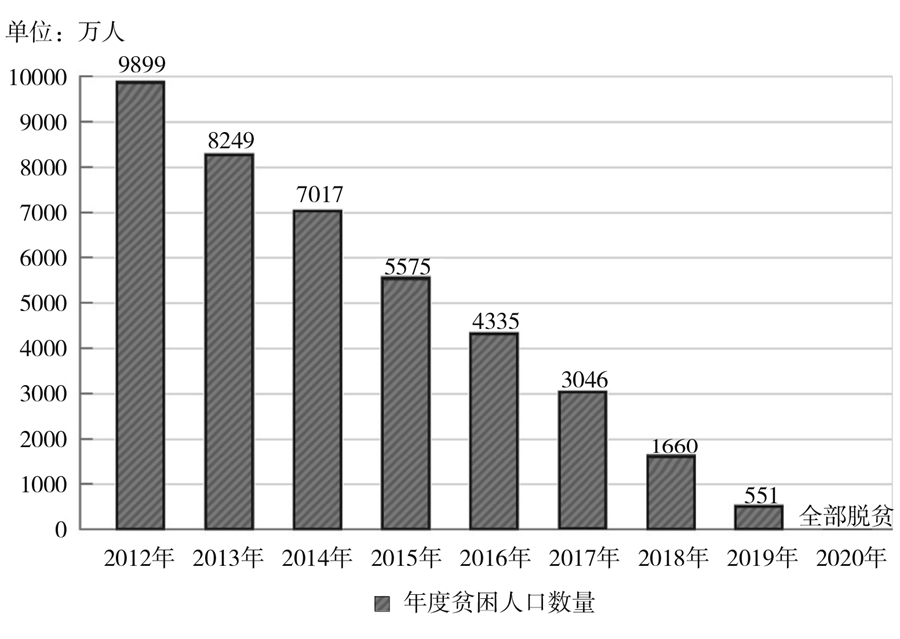
\includegraphics{fig/1.jpg}
    \caption{脱贫攻坚战以来中国农村贫困人口变化情况}
    \label{fig-1}
\end{figure}

\begin{figure}[h]
    \centering
    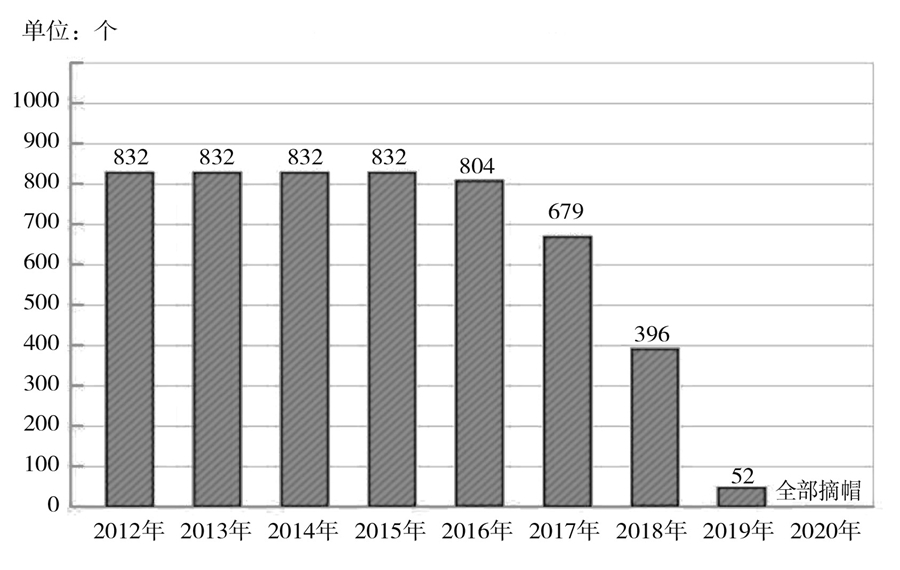
\includegraphics{fig/2.jpg}
    \caption{脱贫攻坚战以来贫困县数量}
    \label{fig-2}
\end{figure}

\subsection{贫困人口生活水平显著提升}

经过脱贫攻坚战,贫困人口的收入和福利水平大幅提高,“两不愁三保障”\endnote{“两不愁三保障”是指稳定实现不愁吃、不愁穿和义务教育、基本医疗、住房安全有保障。}全面实现,教育、医疗、住房、饮水等条件明显改善,既满足了基本生存需要,也为后续发展奠定了基础。脱贫攻坚的阳光照耀到每一个角落,贫困群众的生活发生了巨大变化。

贫困人口收入水平持续提升(图\ref{fig-3})。贫困地区农村居民人均可支配收入,从2013的6079元增长到2020年的12588元,年均增长11.6\%,增长持续快于全国农村,增速比全国农村高2.3个百分点。贫困人口工资性收入和经营性收入占比逐年上升,转移性收入占比逐年下降,自主增收脱贫能力稳步提高。少数民族和民族地区脱贫攻坚成效显著,2016年至2020年,内蒙古自治区、广西壮族自治区、西藏自治区、宁夏回族自治区、新疆维吾尔自治区和贵州、云南、青海三个多民族省份贫困人口累计减少1560万人。28个人口较少民族全部实现整族脱贫,一些新中国成立后“一步跨千年”进入社会主义社会的“直过民族”\endnote{直过民族”是云南省对部分民族的特定称谓,源于这些民族在民主改革时期,跨越一个或几个发展阶段直接进入社会主义社会。},又实现了从贫穷落后到全面小康的第二次历史性跨越。

\begin{figure}[h]
    \centering
    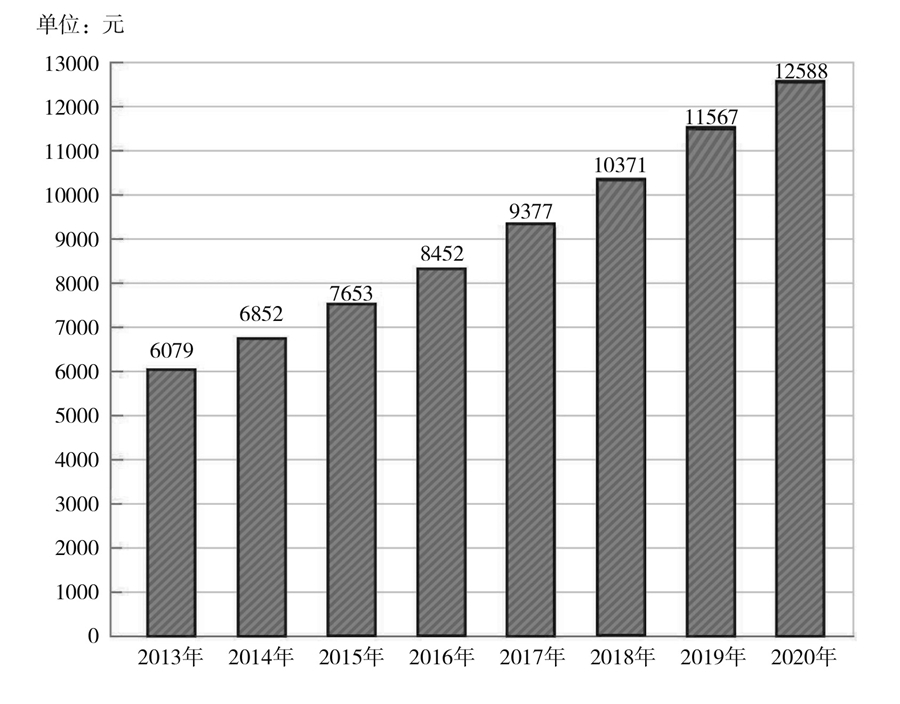
\includegraphics{fig/3.jpg}
    \caption{贫困地区农村居民人均可支配收入}
    \label{fig-3}
\end{figure}

“两不愁三保障”全面实现。脱贫攻坚普查\endnote{脱贫攻坚普查是精准扶贫精准脱贫的重要基础性工作,是对脱贫攻坚成效的全面检验。2020年至2021年,中国在中西部22个省份开展了国家脱贫攻坚普查,重点围绕脱贫结果的真实性和准确性,全面了解国家贫困县脱贫实现情况。普查内容包括建档立卡基本情况、“两不愁三保障”实现情况、获得帮扶和参与脱贫攻坚项目情况,以及县和行政村基本公共服务情况等。}显示,贫困户全面实现不愁吃、不愁穿,平时吃得饱且能适当吃好,一年四季都有应季的换洗衣物和御寒被褥。贫困人口受教育的机会显著增多、水平持续提高,农村贫困家庭子女义务教育阶段辍学问题实现动态清零,2020年贫困县九年义务教育巩固率达到94.8\%。持续完善县乡村三级医疗卫生服务体系,把贫困人口全部纳入基本医疗保险、大病保险、医疗救助三重制度保障范围,实施大病集中救治、慢病签约管理、重病兜底保障等措施,99.9\%以上的贫困人口参加基本医疗保险,全面实现贫困人口看病有地方、有医生、有医疗保险制度保障,看病难、看病贵问题有效解决。实施农村危房改造,贫困人口全面实现住房安全有保障(专栏\ref{col-1})。实施农村饮水安全和巩固提升工程,累计解决2889万贫困人口的饮水安全问题,饮用水量和水质全部达标,3.82亿农村人口受益;贫困地区自来水普及率从2015年的70\%提高到2020年的83\%。

\begin{zhuanlan}[农村危房改造]

农村危房改造是实现“两不愁三保障”的重要举措。2013年以来,累计有790万户2568万贫困人口告别破旧的泥草房、土坯房等危房,住上了安全住房。同时,支持1075万户农村低保户、分散供养特困人员、困难残疾人家庭等改造危房。将贫困地区农村危房改造与改善村容村貌相结合,推进村内道路绿化、安全供水、垃圾污水治理等设施建设,整体人居环境显著提升。具有民族特色、地方特色的贫困地区在进行农村危房改造时最大限度保留传统建筑风格,打造出一批旅游村、文化村,实现了增收致富。

国家提供资金补助,帮助农村贫困群众改造危房。从2017年起,中央财政户均补助标准从8500元提高到1.4万元。地方统筹各级财政补助资金,并根据农户贫困程度、房屋危险程度和改造方式等制定分级分类补助标准,保证了贫困户建得起基本安全的住房。对于部分鳏寡孤独等无力改造住房的特困群众,通过统建农村集体公租房及幸福大院、修缮加固现有闲置公房、置换或长期租赁村内闲置农房等方式,兜底解决住房安全问题。

\label{col-1}

\end{zhuanlan}

\subsection{贫困地区落后面貌根本改变}

长期以来,贫困地区基础设施薄弱,公共服务匮乏,经济社会发展滞后。脱贫攻坚战不仅使农村贫困人口全部脱贫,而且使贫困地区经济社会发展大踏步赶上来,整体面貌发生历史性巨变。

基础设施显著改善。出行难、用电难、用水难、通信难,是长期以来制约贫困地区发展的瓶颈。把基础设施建设作为脱贫攻坚基础工程,集中力量,加大投入,全力推进,补齐了贫困地区基础设施短板,推动了贫困地区经济社会快速发展。以建好、管好、护好、运营好农村公路(简称“四好农村路”,专栏\ref{col-2})为牵引,积极推进贫困地区建设外通内联、通村畅乡、客车到村、安全便捷的交通运输网络。截至2020年底,全国贫困地区新改建公路110万公里、新增铁路里程3.5万公里,贫困地区具备条件的乡镇和建制村全部通硬化路、通客车、通邮路,贫困地区因路而兴、因路而富。努力改善贫困地区水利基础设施条件,2016年以来,新增和改善农田有效灌溉面积8029万亩,新增供水能力181亿立方米,水利支撑贫困地区发展的能力显著增强。大幅提升贫困地区用电条件,实施无电地区电力建设、农村电网改造升级、骨干电网和输电通道建设等电网专项工程,把电网延伸到更多偏远地区,农村地区基本实现稳定可靠的供电服务全覆盖,供电能力和服务水平明显提升(专栏\ref{col-3})。加强贫困地区通信设施建设,贫困村通光纤和4G比例均超过98\%,远程教育加快向贫困地区学校推进,远程医疗、电子商务覆盖所有贫困县,贫困地区信息化建设实现跨越式发展。基础设施的极大改善,从根本上破解了贫困地区脱贫致富的难题,畅通了贫困地区与外界的人流、物流、知识流、信息流,为贫困地区发展提供了有力的硬件支撑。

\begin{zhuanlan}[“四好农村路”]
    “四好农村路"是新时代中国农村变化和社会变迁的重要标志。截至2019年底,农村公路总里程占全国公路总里程的83.8\%,其中等级公路比例达到93.29\%,农村公路列养率达到98.8\%。贫困地区改造建设约5.9万公里资源路、旅游路、产业路,出行难等长期没有解决的老大难问题普遍得到解决。 “四好农村路"连片成网,极大缩短了往返城乡距离,深刻改变了农村的生产生活条件和社会面貌,为偏远闭塞的乡村开辟了通往现代化的大道。
    \label{col-2}
\end{zhuanlan}

\begin{zhuanlan}[加强贫困地区电力供应和保障]
    农村电网是农村经济社会发展的重要基础设施。2013年以来,中国实施全面解决无电人口用电问题三年行动计划,到2015年实现了全国人口用上电。通过实施新一轮农网改造升级,农网供电可靠率达到99.8\%、综合电压合格率达到99.7\%,农村居民用电条件明显改善。2020年底,实现了全国县级行政区全部接入大电网。实施贫困村通动力电工程,覆盖23个省份839个县约17万个行政村,大电网覆盖范围内贫困村通动力电比例达到100\%。
    \label{col-3}
\end{zhuanlan}

基本公共服务水平明显提升。在解决好贫困人口吃饭、穿衣、居住等温饱问题基础上,大力提升贫困地区教育、医疗、文化、社会保障等基本公共服务水平,实现贫困人口学有所教、病有所医、老有所养、弱有所扶,为贫困地区发展夯实基础、积蓄后劲。2013年以来,累计改造贫困地区义务教育薄弱学校10.8万所,实现贫困地区适龄儿童都能在所在村上幼儿园和小学。贫困地区公共文化服务水平不断提高,截至2020年底,中西部22个省份基层文化中心建设完成比例达到99.48\%,基本实现村级文化设施全覆盖;持续推进文化下乡,贫困群众也有了丰富多彩的业余文化生活。贫困地区医疗条件显著改善,消除了乡村两级医疗卫生机构和人员“空白点”,98\%的贫困县至少有一所二级以上医院,贫困地区县级医院收治病种中位数达到全国县级医院整体水平的90\%,贫困人口的常见病、慢性病基本能够就近获得及时诊治,越来越多的大病在县域内就可以得到有效救治。综合保障体系逐步健全,贫困县农村低保标准全部超过国家扶贫标准,1936万贫困人口纳入农村低保或特困救助供养政策;6098万贫困人口参加了城乡居民基本养老保险,基本实现应保尽保。

经济持续快速发展。脱贫攻坚极大释放了贫困地区蕴含的潜力,为经济发展注入强大动力。产业结构显著改善,特色优势产业不断发展,电子商务、光伏、旅游等新业态新产业蓬勃兴起,推动了贫困地区经济多元化发展,扩大了市场有效供给,厚植了经济发展基础。贫困地区的地区生产总值持续保持较快增长,2015年以来,人均一般公共预算收入年均增幅高出同期全国平均水平约7个百分点。收入的持续稳定增长,激发了贫困群众提升生活品质、丰富精神文化生活的需求,拉动了庞大的农村消费,为促进国内大循环提供了支撑。

优秀文化传承弘扬。加强贫困地区传统文化、特色文化、民族文化的保护、传承和弘扬,贫困地区优秀文化繁荣发展。实施国家传统工艺振兴工程,引导和推动革命老区、民族地区、边疆地区、贫困地区保护好、发展好当地优秀传统技艺。支持贫困地区深入挖掘民族文化、红色文化、乡土文化、非物质文化遗产特色资源,加强保护研究、人才培养、展示推广,打造特色文化旅游产业。开展留存扶贫印记活动,建立贫困村扶贫档案,鼓励支持扶贫题材影视文艺作品创作,生动记录脱贫致富历程。贫困地区优秀文化的保护传承,既促进了贫困群众增收致富,也延续了文脉、留住了乡愁。

生态环境更美更好。将扶贫开发与水土保持、环境保护、生态建设相结合,通过生态扶贫、农村人居环境整治、生态脆弱地区易地扶贫搬迁等措施,贫困地区生态保护水平明显改善,守护了绿水青山、换来了金山银山。脱贫攻坚既促进了贫困人口“增收”,又促进了贫困地区“增绿”,极大改善了贫困地区生态环境,广大农村旧貌换了新颜,生态宜居水平不断提高。

深度贫困地区是贫中之贫、坚中之坚。通过脱贫攻坚,“三区三州”\endnote{“三区”是指:西藏自治区、新疆维吾尔自治区南疆四地州和四川省、云南省、甘肃省、青海省涉藏州县。“三州”是指:四川省凉山彝族自治州、云南省怒江傈僳族自治州和甘肃省临夏回族自治州。}等深度贫困地区突出问题得到根本解决,基础设施和公共服务水平显著提升,特色主导产业加快发展,社会文明程度明显提高,区域性整体贫困问题彻底解决(专栏\ref{col-4})。

\begin{zhuanlan}[深度贫困地区脱贫攻坚]
    深度贫困地区脱贫攻坚是事关脱贫攻坚战成败的硬骨头,是影响全面建成小康社会的最大短板。2017年6月23日,习近平总书记主持召开深度贫困地区脱贫攻坚座谈会,强调要加快推进深度贫困地区脱贫攻坚。会后,印发《关于支持深度贫困地区脱贫攻坚的实施意见》,明确新增脱贫攻坚资金、项目、举措主要用于深度贫困地区,国家重点支持“三区三州”。相关省份制定实施方案,相关县制定具体方案。有关部门制定49个专项政策文件,涵盖财政、金融、土地、住房、教育、医疗、生态 、产业、水利等领域。2018-2020年,中央财政对深度贫困地区新增资金722亿元,占三年新增资金总量的60.2\%。中央优先安排公益性基础设施项目、社会事业领域重大工程建设项目以及能源、交通等重大投资项目。2017年以来,每年专项安排每县600亩用地计划指标。2018年以来,累计下达深度贫困地区所在省土地增减挂跨省交易节余指标61.8万亩,筹资约1900亿元。实行差异化信贷支持政策,适度提高创业、担保、贷款、贴息额度,提高个人精准扶贫贷款不良率容忍度,取消反担保要求。对“三区三州”符合条件的企业首次公开发行股票,适用“即报即审、审过即发”政策。
    \label{col-4}
\end{zhuanlan}

\subsection{脱贫群众精神风貌焕然一新}

脱贫攻坚既是一场深刻的物质革命,也是一场深刻的思想革命;既取得了物质上的累累硕果,也取得了精神上的累累硕果。贫困群众的精神世界在脱贫攻坚中得到充实和升华,信心更坚、脑子更活、心气更足,发生了从内而外的深刻改变。

脱贫致富热情高涨。脱贫攻坚不仅使贫困群众拓宽了增收渠道、增加了收入,而且唤醒了贫困群众对美好生活的追求,极大提振和重塑了贫困群众自力更生、自强不息,勤劳致富、勤俭持家,创业干事、创优争先的精气神,增强了脱贫致富的信心和劲头。“好日子是干出来的”,贫困群众比着把日子往好里过,依靠自己的辛勤劳动摆脱贫困,形成了你追我赶奔小康的浓厚氛围。

主人翁意识显著提升。脱贫攻坚为贫困群众参与集体事务搭建了新的平台。扶贫项目实施、资金使用等村级重大事项决策,实行“四议两公开”\endnote{“四议两公开”,是指在村党组织领导下对村级事务进行民主决策的基本工作程序。“四议”指党支部会提议、村“两委”会商议、党员大会审议、村民代表会议或村民会议决议;“两公开”指决议公开、实施结果公开。},建立健全村务监督机制,推广村民议事会、扶贫理事会等制度,让村民做到“大家的事大家议、大家办”,拓展了贫困群众参与脱贫攻坚的议事管事空间,提高了参与集体事务的积极性自觉性,激发了建设家乡的热情,乡村发展的凝聚力大大增强。

现代观念不断增强。脱贫攻坚打开了贫困地区通往外部世界的大门。交通基础设施的改善打通了贫困地区与外界的联系,公共文化事业的发展丰富了贫困群众的精神文化生活,网络的普及让贫困群众增长了见识、开阔了视野。贫困群众的开放意识、创新意识、科技意识、规则意识、市场意识等显著增强,脱贫致富的点子越来越多、路子越来越宽。

文明新风广泛弘扬。深化贫困地区文明村镇和文明家庭、“五好”家庭创建,持续推进新时代文明实践中心建设,发挥村规民约作用,推广道德评议会、红白理事会等做法,开展移风易俗行动,开展弘扬好家风、“星级文明户”评选、寻找“最美家庭”等活动,社会主义核心价值观广泛传播,贫困地区文明程度显著提升。俭朴节约、绿色环保、讲究卫生等科学、健康、文明的生活方式成为贫困群众的新追求,婚事新办、丧事简办、孝亲敬老、邻里和睦、扶危济困、扶弱助残等社会风尚广泛弘扬,既有乡土气息又有现代时尚的新时代乡村文明新风正在形成。

\subsection{特殊困难群体生存发展权利有效保障}

中国高度重视妇女、儿童、老人和残疾人等群体中特殊困难人员的生存和发展,采取特殊政策,加大帮扶力度,特殊困难群体的福利水平持续提高,生存权利充分保障,发展机会明显增多。

贫困妇女生存发展状况显著改善。坚持男女平等基本国策,将妇女作为重点扶贫对象,实现脱贫的近1亿贫困人口中妇女约占一半。实施《中国妇女发展纲要(2011-2020年)》,把缓解妇女贫困程度、减少贫困妇女数量放在优先位置,扶贫政策、资金、措施优先向贫困妇女倾斜,帮助贫困妇女解决最困难最忧虑最急迫的问题。累计对1021万名贫困妇女和妇女骨干进行各类技能培训,500多万名贫困妇女通过手工、种植养殖、家政、电商等增收脱贫。累计发放妇女小额担保贷款和扶贫小额信贷4500多亿元,870万名妇女通过小额担保贷款和扶贫小额信贷实现创业增收。19.2万名贫困患病妇女获得救助,妇女宫颈癌、乳腺癌免费检查项目在贫困地区实现全覆盖。通过“母亲水窖”“母亲健康快车”“母亲邮包”等公益项目,投入公益资金41.7亿元,惠及贫困妇女5000余万人次。

困境儿童关爱水平明显提高。实施《中国儿童发展纲要(2011-2020年)》《国家贫困地区儿童发展规划(2014-2020年)》,对儿童教育和健康实施全过程保障和干预。开展儿童营养知识宣传和健康教育,实施贫困地区儿童营养改善项目,提高贫困地区儿童健康水平,为集中连片特困地区6-24月龄婴幼儿每天免费提供1包辅食营养补充品,截至2020年底,累计1120万儿童受益。实施出生缺陷干预救助项目,为先天性结构畸形、部分遗传代谢病和地中海贫血贫困患病儿童提供医疗费用补助,累计救助患儿4.1万名,拨付救助金4.7亿元。组织各类志愿者与孤儿、农村留守儿童、困境儿童结对,开展关爱帮扶,覆盖儿童和家长2519.2万人次。建立儿童之家28万余所、儿童快乐家园1200余个,为留守、困境儿童提供文体娱乐、心理疏导、生活照顾、家教指导等关爱服务。大幅提高孤儿保障水平,机构集中养育孤儿和社会散居孤儿平均保障标准分别达到每人每月1611.3元和1184.3元。实施孤儿医疗康复明天计划项目,累计投入17亿元、惠及22.3万名病残孤儿。实施福彩梦圆孤儿助学工程,累计投入5.4亿元、惠及在校就读孤儿5.4万人次。建立事实无人抚养儿童保障制度,25.3万名事实无人抚养儿童参照当地孤儿保障标准纳入保障范围。

贫困老年人生活和服务保障显著改善。持续提高农村养老金待遇和贫困老年人口医疗保障水平,农村老年人口贫困问题进一步解决。经济困难的高龄、失能等老年人补贴制度全面建立,惠及3689万老年人。实施老年健康西部行项目,在西部贫困地区开展老年健康宣传教育,组织医务人员、志愿者开展义诊和健康指导服务,促进西部老年人健康素养和健康水平提高。建立农村留守老年人关爱服务制度,推动贫困老年人医疗保障从救治为主向健康服务为主转变。加强失能贫困老年人关爱照护,全面开展核查,确认62.7万失能贫困老年人,落实家庭医生签约服务59万人,失能贫困老年人健康状况明显改善。

贫困残疾人保障水平全面提升。700多万贫困残疾人如期脱贫,创造了人类减贫史上残疾人特殊困难群体消除贫困的奇迹。困难残疾人生活补贴和重度残疾人护理补贴制度惠及2400多万残疾人。1066.7万残疾人纳入最低生活保障。贫困残疾人全部纳入基本医疗保险、大病保险,54.7万贫困残疾人得到医疗救助。178.5万户贫困残疾人家庭住房安全问题得到解决。贫困残疾人的特殊需求得到更好保障,8万余名家庭经济困难的残疾儿童接受普惠性学前教育。65.3万户贫困重度残疾人家庭完成无障碍改造,贫困重度残疾人照护服务创新实践取得显著成效。

\subsection{贫困地区基层治理能力显著提升}

脱贫攻坚是国家治理体系和治理能力现代化在贫困治理领域的成功实践。打赢脱贫攻坚战,促进了国家贫困治理体系的完善,贫困地区基层治理体系进一步健全、治理能力显著提升。

农村基层党组织更加坚强。农村基层党组织是中国共产党在农村全部工作和战斗力的基础,是贯彻落实扶贫工作决策部署的战斗堡垒。坚持抓党建促脱贫攻坚、抓扶贫先强班子,整顿软弱涣散基层党组织,精准选派贫困村党组织第一书记、驻村工作队,把农村致富能手、退役军人、外出务工经商返乡人员、农民合作社负责人、大学生村官等群体中具有奉献精神、吃苦耐劳、勇于创新的优秀党员选配到村党组织书记岗位上,基层党组织的战斗堡垒作用不断增强,凝聚力战斗力号召力明显提高,党群干群关系更加密切,贫困地区群众对党和政府的信赖、信任、信心进一步增强,党在农村的执政基础更加牢固。

基层群众自治更加有效。脱贫攻坚有力推动了贫困地区基层民主政治建设,基层治理更具活力。村委会(居委会)作用更好发挥,贫困群众自我管理、自我教育、自我服务、自我监督不断加强。认真落实村(居)务公开,坚持重大问题民主决策。坚持群众的事由群众商量着办,群众的事由群众定,群众参与基层治理的积极性主动性创造性进一步增强。脱贫攻坚之初,很多贫困村几乎没有集体经济收入,到2020年底全国贫困村的村均集体经济收入超过12万元。稳定的集体经济收入改变了很多村级组织过去没钱办事的困境,增强了村级组织自我保障和服务群众的能力。

懂农业、爱农村、爱农民的“三农”工作队伍不断壮大。2013年以来,全国累计选派300多万名第一书记和驻村干部开展精准帮扶。广大基层干部和扶贫干部心系贫困群众、甘愿牺牲奉献,满腔热情地为贫困群众办实事、解难题,赢得了贫困群众发自内心的认可。在脱贫攻坚的艰苦磨砺中,广大基层干部和扶贫干部坚韧、乐观、充满奋斗精神,带领群众脱贫致富的信心更加坚定、本领进一步增强。大批教育、科技、医疗卫生、文化等领域的专业人才支援贫困地区建设,大批企业家到贫困地区投资兴业,很多高校毕业生放弃城市的优厚待遇回到农村建设家乡。变富变美的农村吸引力不断增强,大批热爱农村、扎根农村、建设农村的人才留下来,为农业农村现代化继续贡献力量。

社会治理水平明显提升。脱贫攻坚为贫困地区带来了先进发展理念、现代科技手段、科学管理模式,显著提升了贫困地区的社会治理水平。脱贫攻坚行之有效的制度体系和方法手段,为基层社会治理探索了新路径,促进了网格化管理、精细化服务、信息化支撑、开放共享的基层管理服务体系的建立和完善,社会治理的社会化、法治化、智能化、专业化水平进一步提升,基层社会矛盾预防和化解能力显著增强,贫困地区社会更加和谐、稳定、有序。

脱贫攻坚战取得全面胜利,创造了中国减贫史乃至人类减贫史上的伟大奇迹,极大增强了中华民族的自信心自豪感和凝聚力向心力,极大增强了中国人民的道路自信、理论自信、制度自信、文化自信,极大增强了中国人民创造更加美好生活的信心和底气。这一伟大胜利,彰显了中国共产党始终坚守的初心使命和强大政治领导力、思想引领力、群众组织力、社会号召力,彰显了中国特色社会主义制度集中力量办大事的优势,彰显了中国精神、中国价值、中国力量,彰显了中国人民为实现梦想拼搏奋斗、敢教日月换新天的意志品质,彰显了中华民族无所畏惧、不屈不挠、敢于斗争、坚决战胜前进道路上一切困难和挑战的精神品格。脱贫攻坚伟大实践锻造形成“上下同心、尽锐出战、精准务实、开拓创新、攻坚克难、不负人民”的脱贫攻坚精神,赓续传承了伟大民族精神和时代精神,将激励中国人民为创造美好未来继续奋斗。

\section{实施精准扶贫方略}

对于贫困人口规模庞大的国家,找准贫困人口、实施扶真贫是普遍性难题。脱贫攻坚贵在精准、重在精准,成败之举在于精准。中国在脱贫攻坚实践中,积极借鉴国际经验,紧密结合中国实际,创造性地提出并实施精准扶贫方略,做到扶持对象、项目安排、资金使用、措施到户、因村派人、脱贫成效“六个精准”,实施发展生产、易地搬迁、生态补偿、发展教育、社会保障兜底“五个一批”,解决好扶持谁、谁来扶、怎么扶、如何退、如何稳“五个问题”,增强了脱贫攻坚的目标针对性,提升了脱贫攻坚的整体效能。

\subsection{精准识别、建档立卡,解决“扶持谁”的问题}

扶贫必先识贫。中国贫困人口规模大、结构复杂,实现精准扶贫首先要精准识贫。科学制定贫困识别的标准和程序,组织基层干部进村入户,摸清贫困人口分布、致贫原因、帮扶需求等情况。贫困户识别以农户收入为基本依据,综合考虑住房、教育、健康等情况,通过农户申请、民主评议、公示公告、逐级审核的方式,进行整户识别;贫困村识别综合考虑行政村贫困发生率、村民人均纯收入和村集体经济收入等情况,按照村委会申请、乡政府审核公示、县级审定公告等程序确定。对识别出的贫困村和贫困人口建档立卡,建立起全国统一的扶贫信息系统。组织开展“回头看”,实行动态管理,及时剔除识别不准人口、补录新识别人口,提高识别准确率。建档立卡在中国扶贫史上第一次实现贫困信息精准到村到户到人,精确瞄准了脱贫攻坚的对象,第一次逐户分析致贫原因和脱贫需求,第一次构建起国家扶贫信息平台,为实施精准扶贫精准脱贫提供了有力的数据支撑。

\subsection{加强领导、建强队伍,解决“谁来扶”的问题}

脱贫攻坚涉及面广、要素繁多、极其复杂,需要强有力的组织领导和贯彻执行。充分发挥党的政治优势、组织优势,建立中央统筹、省负总责、市县抓落实的脱贫攻坚管理体制和片为重点、工作到村、扶贫到户的工作机制,构建起横向到边、纵向到底的工作体系。各级党委充分发挥总揽全局、协调各方的作用,执行脱贫攻坚一把手负责制,中西部22个省份党政主要负责同志向中央签署责任书、立下军令状,省市县乡村五级书记一起抓。脱贫攻坚期内,贫困县党委政府正职保持稳定。有脱贫任务的地区,倒排工期、落实责任,抓紧施工、强力推进。脱贫攻坚任务重的地区,把脱贫攻坚作为头等大事和第一民生工程,以脱贫攻坚统揽经济社会发展全局。实行最严格的考核评估和监督检查,组织脱贫攻坚专项巡视,开展扶贫领域腐败和作风问题专项治理(专栏\ref{col-5}),加强脱贫攻坚督导和监察(专栏\ref{col-6}),确保扶贫工作务实、脱贫过程扎实、脱贫结果真实,使脱贫攻坚成果经得起实践和历史检验。建立健全干部担当作为的激励和保护机制,加大关心关爱干部力度,树立正确用人导向,引导广大干部在决胜脱贫攻坚中奋发有为、履职尽责。加强基层扶贫队伍建设,普遍建立干部驻村帮扶工作队制度,按照因村派人、精准选派的原则,选派政治素质好、工作能力强、作风实的干部驻村扶贫。广大驻村干部牢记使命、不负重托,心系贫困群众,扎根基层扶贫一线,倾心倾力帮助贫困群众找出路、谋发展、早脱贫。从2013年开始向贫困村选派第一书记和驻村工作队,到2015年,实现每个贫困村都有驻村工作队、每个贫困户都有帮扶责任人。截至2020年底,全国累计选派25.5万个驻村工作队、300多万名第一书记和驻村干部,同近200万名乡镇干部和数百万村干部一道奋战在扶贫一线。

\begin{zhuanlan}[坚决查处脱贫攻坚中的违规违纪问题]
    中央纪委国家监委机关开展扶贫领域监督执纪问责工作、扶贫领域腐败和作风问题专项治理,坚决查处违规违纪问题,为脱贫攻坚营造了良好的干事创业环境和风清气正氛围。中共十八大以来,对498件扶贫领域典型问题线索进行督办,查实率87\%,对相关责任人进行严肃追责问责,通报曝光69起扶贫领域腐败和作风问题典型案例。2016年1月至2020年11月,全国纪检监察机关查处扶贫领域腐败和作风问题33.77万个,批评教育帮助和处理46.45万人,其中给予党纪政务处分24.13万人。
    \label{col-5}
\end{zhuanlan}

\begin{zhuanlan}[脱贫攻坚监督体系]
    加强脱贫攻坚督导监察,建立党内与党外相结合、政府与社会相结合的全方位监督体系,有效防止弄虚作假、贪污腐败等问题。

    党内监督:运用巡视利器,将脱贫攻坚纳入巡视范围。十九届中共中央第一轮巡视将脱贫攻坚工作纳入14个巡视省份监督内容。十九届中共中央第二轮巡视对13个省(自治区、直辖市) 以及脱贫攻坚中承担重要职责的11个中央国家机关和2家中央人金融企业的党组织进行脱贫攻坚专项巡视。

    民主监督:从2016年开始,受中共中央委托,8个民主党派中央对口8个脱贫攻坚任务重的省份开展民主监督,深入对口地方一线调查研究,对脱贫攻坚落实情况进行监督。这是民主党派首次对国家重大战略开展专项监督,也是民主党派开展的规模最大、时间跨度最长的专项监督活动。

    督查巡查:2016年以来,原国务院扶贫开发领导小组每年开展一次脱贫攻坚督查巡查,重点对中西部22个省份党委和政府、中央和国家机关有关单位脱贫攻坚工作进行督查和巡查。

    审计监督:审计署每年持续组织实施脱贫攻坚政策措施落实和重点资金项目跟踪审计,实现了对832个贫困县的扶贫审计全覆盖。审计查出扶贫资金问题金额占抽查资金比例由2013年的36.3\%下降至2020年的1.5\%。

    行业监督:发展改革、财政、教育、住房建设、卫生健康、医疗保障、水利等部门围绕脱贫攻坚政策举措和任务落实加强行业监督。

    社会监督:2014年12月开通12317扶贫监督举报电话,接受社会监督,主要受理对扶贫资金管理、分配、使用中的问题,扶贫项目实施管理中的问题以及挤占、贪污、挪用扶贫资金等行为的反映和投诉。新闻媒体加大监督力度,及时曝光脱贫攻坚中存在的问题,提出建设性意见和建议。
    \label{col-6}
\end{zhuanlan}

\subsection{区分类别、靶向施策,解决“怎么扶”的问题}

贫困的类型和原因千差万别,开对“药方子”才能拔掉“穷根子”。中国在减贫实践中,针对不同情况分类施策、对症下药,因人因地施策,因贫困原因施策,因贫困类型施策,通过实施“五个一批”实现精准扶贫。

发展生产脱贫一批。发展产业是脱贫致富最直接、最有效的办法,也是增强贫困地区造血功能、帮助贫困群众就地就业的长远之计。支持和引导贫困地区因地制宜发展特色产业,鼓励支持电商扶贫、光伏扶贫、旅游扶贫等新业态新产业发展(专栏\ref{col-7}),依托东西部扶贫协作推进食品加工、服装制造等劳动密集型产业梯度转移,一大批特色优势产业初具规模,增强了贫困地区经济发展动能。累计建成各类产业基地超过30万个,形成了特色鲜明、带贫面广的扶贫主导产业,打造特色农产品品牌1.2万个。发展市级以上龙头企业1.44万家、农民合作社71.9万家,72.6\%的贫困户与新型农业经营主体建立了紧密型的利益联结关系。产业帮扶政策覆盖98.9\%的贫困户,有劳动能力和意愿的贫困群众基本都参与到产业扶贫之中。扎实推进科技扶贫,建立科技帮扶结对7.7万个,选派科技特派员28.98万名,投入资金200多亿元,实施各级各类科技项目3.76万个,推广应用先进实用技术、新品种5万余项,支持贫困地区建成创新创业平台1290个。为贫困户提供扶贫小额信贷支持(专栏\ref{col-8}),培育贫困村创业致富带头人,建立完善带贫机制,鼓励和带领贫困群众发展产业增收致富。

\begin{zhuanlan}[光伏扶贫和电商扶贫]
    光伏扶贫电站是以扶贫为目的,在具备光伏扶贫实施条件的地区,利用政府性资金投资建设的光伏电站,其产权归村集体所有,全部收益用于扶贫。截至2020年底,全国光伏扶贫容量达到1865万千瓦,10万个村有村级电站,村年均收益20万元左右,主要用于设立公益岗位、实施小型公益项目、开展小微奖励补助等。
    
    积极推进电商扶贫工程,充分发掘电商带动贫困群众增收的潜力,取得显著成效。2014年起在全国开展电子商务进农村综合示范工作,实现对832个贫困县的全覆盖,到2020年底累计投入资金249.17亿元,贫困县网商从2016年的131.5万家增长到2020年的311.23万家。甘肃省陇南市在电商扶贫方面走在全国前列,截至2020年,全市共开办网店1.4万家,累计销售220多亿元,带动50万贫困群众实现增收,电商扶贫对贫困户人均贡献额从2015年的430元增长到2020年的930元。
    \label{col-7}
\end{zhuanlan}

\begin{zhuanlan}[扶贫小额信贷]
    为解决贫困群众贷款难、贷款贵问题,2014年,中国创新推出专门针对贫困群众的信贷产品——扶贫小额信贷,其特点是“5万元以下3年期以内、免担保免抵押、基准利率放贷、财政贴息、县建风险补偿金”。扶贫小额信贷瞄准贫困户发展生产的薄弱环节,将金融活水引入贫困地区,调动了贫困户创业增收的积极性,同时,增强了贫困群众的市场意识、风险防范意识和信用意识,激活了内生发展动力,增加了农村金融有效供给。截至2020年底,全国扶贫小额信贷累计发放7100多亿元,累计支持贫困户1500多万户。
    \label{col-8}
\end{zhuanlan}

易地搬迁脱贫一批。对生活在自然环境恶劣、生存条件极差、自然灾害频发地区,很难实现就地脱贫的贫困人口,实施易地扶贫搬迁(专栏\ref{col-9})。充分尊重群众意愿,坚持符合条件和群众自愿原则,加强思想引导,不搞强迫命令。全面摸排搬迁对象,精心制定搬迁规划,合理确定搬迁规模,有计划有步骤稳妥实施。960多万生活在“一方水土养不好一方人”地区的贫困人口通过易地搬迁实现脱贫。对搬迁后的旧宅基地实行复垦复绿,改善迁出区生态环境。加强安置点配套设施和产业园区、扶贫车间等建设,积极为搬迁人口创造就业机会,保障他们有稳定的收入,同当地群众享受同等的基本公共服务,确保搬得出、稳得住、逐步能致富。

\begin{zhuanlan}[易地扶贫搬迁]
    易地扶贫搬迁政策性强、难度大,是一项复杂的系统工程。截至2020年底,全国易地扶贫搬迁规划建设任务全面完成,累计建成集中安置区约3.5万个,建设安置住房266万余套,960多万易地搬迁贫困人口全部入住并实现脱贫。新建或改扩建中小学和幼儿园6100多所、医院和社区卫生服务中心1.2万多所、养老服务设施3400余个文化活动场所4万余个。加强后续扶持工作,出台就业帮扶、金融支持、社区管理等一系列具体支持政策措施,易地扶贫搬迁贫困人口中劳动力就业比例达到73.7\%,搬迁贫困家庭中有劳动力家庭就业比例达到94.1\%。
    \label{col-9}
\end{zhuanlan}

生态补偿脱贫一批。践行“绿水青山就是金山银山”理念,坚持脱贫攻坚与生态保护并重,在加大贫困地区生态保护修复力度的同时,增加重点生态功能区转移支付,不断扩大政策实施范围,让有劳动能力的贫困群众就地转为护林员等生态保护人员。2013年以来,贫困地区实施退耕还林还草7450万亩,选聘110多万贫困群众担任生态护林员,建立2.3万个扶贫造林(种草)专业合作社(队)。贫困群众积极参与国土绿化、退耕还林还草等生态工程建设和森林、草原、湿地等生态系统保护修复工作,发展木本油料等经济林种植及森林旅游,不仅拓宽了增收渠道,也明显改善了贫困地区生态环境,实现了“双赢”。

发展教育脱贫一批。坚持再穷不能穷教育、再穷不能穷孩子,加强教育扶贫,不让孩子输在起跑线上,努力让每个孩子都有人生出彩的机会,阻断贫困代际传递(专栏\ref{col-10})。持续提升贫困地区学校、学位、师资、资助等保障能力,20多万名义务教育阶段的贫困家庭辍学学生全部返校就读,全面实现适龄少年儿童义务教育有保障。实施定向招生、学生就业、职教脱贫等倾斜政策,帮助800多万贫困家庭初高中毕业生接受职业教育培训、514万名贫困家庭学生接受高等教育,重点高校定向招收农村和贫困地区学生70多万人,拓宽贫困学生纵向流动渠道。开展民族地区农村教师和青壮年农牧民国家通用语言文字培训,累计培训350万余人次,提升民族地区贫困人口就业能力。“学前学会普通话”行动先后在四川省凉山彝族自治州和乐山市马边彝族自治县、峨边彝族自治县、金口河区开展试点,覆盖43万学龄前儿童,帮助他们学会普通话。

\begin{zhuanlan}[教育扶贫]
    脱贫攻坚战以来,贫困地区办学条件明显改善,全国99.8\%义务教育学校(含教学点)办学条件达到基本要求;贫困地区学校网络普及率大幅提升,全国中小学(含教学点)互联网接人率达到100\%,拥有多媒体教室的学校比例达到95.3\%;乡村教师队伍水平整体提升,“特岗计划”实施以来累计招聘教师95万名,“国培计划”培训中西部乡村学校教师近1700万余人次,连片特困地区乡村教师生活补助惠及8万多所学校127万名教师,累计选派19万名乡村教师到边远贫困地区、边疆民族地区支教;建立了履盖从学前至研究生各个教育阶段的资助体系,累计资助6.4亿人次;义务教育营养改善计划覆盖1634个县、13.63万所学校、每年惠及4000余万名学生。
    \label{col-10}
\end{zhuanlan}

社会保障兜底一批。聚焦特殊贫困群体,落实兜底保障政策。实施特困人员供养服务设施改造提升工程,集中供养能力显著增强。农村低保制度与扶贫政策有效衔接,全国农村低保标准从2012年每人每年2068元提高到2020年5962元,提高188.3\%。扶贫部门与民政部门定期开展数据比对、摸排核实,实现贫困人口“应保尽保”。

中国还结合实际、因地制宜,采取其他多渠道多元化扶贫措施。大力推进就业扶贫,通过免费开展职业技能培训、东西部扶贫协作劳务输出、扶贫车间和扶贫龙头企业吸纳、返乡创业带动、扶贫公益性岗位安置等形式,支持有劳动能力的贫困人口在本地或外出务工、创业,贫困劳动力务工规模从2015年的1227万人增加到2020年的3243万人。开展健康扶贫工程,把健康扶贫作为脱贫攻坚重要举措,防止因病致贫返贫(专栏\ref{col-11})。深入实施网络扶贫工程,支持贫困地区特别是“三区三州”等深度贫困地区,完善网络覆盖,推进“互联网+”扶贫模式。实施资产收益扶贫,把中央财政专项扶贫资金和其他涉农资金投入设施农业、光伏、乡村旅游等项目形成的资产,折股量化到贫困村,推动产业发展,增加群众收入,破解村集体经济收入难题。2020年新冠肺炎疫情发生后,中国采取一系列应对疫情的帮扶举措,加大就业稳岗力度,开展消费扶贫行动,有效克服了新冠肺炎疫情影响。

\begin{zhuanlan}[健康扶贫]
    加强县乡村三级医疗卫生机构和人才队伍建设,组织1007家三级医院与1172家贫困地区县级医院结对帮扶,累计派出超过11.8万人次医务人员,帮助贫困地区新建临床重点专科超过3700个,开展新技术、新项目超过5.3万项,门诊诊疗人次超过5500万,管理出院患者超过600万,完成住院、门诊手术超过190万台。倾斜实施农村订单定向医学生免费培养项目,累计培养6万余名医学生,3万余名顺利毕业并赴各乡镇卫生院履约。大力实施全科医生特岗计划,累计招聘特岗医生5000余人,目前,贫困地区有近5万名全科医生。指导地方通过“县聘县管乡用”“乡聘村用”以及巡诊派驻等灵活方式,累计支援乡村两级医务人员近10万人。远程医疗覆盖所有贫困县并快速向乡镇卫生院延伸。坚持预防为主、强化重大疾病综合防控和重点人群健康改善,深入开展爱国卫生运动和健康促进行动。实施“三区三州”传染病地方病防治攻坚行动,长期影响当地群众身体健康的传染病、地方病等重大疾病基本消除或有效控制。
    \label{col-11}
\end{zhuanlan}

\subsection{严格标准、有序退出,解决“如何退”的问题}

建立贫困退出机制,明确贫困县、贫困村、贫困人口退出的标准和程序,既防止数字脱贫、虚假脱贫等“被脱贫”,也防止达到标准不愿退出等“该退不退”。制定脱贫摘帽规划和年度减贫计划,确保规范合理有序退出。严格执行退出标准,严格规范工作流程,贫困人口退出实行民主评议,贫困村、贫困县退出进行审核审查,退出结果公示公告,让群众参与评价,做到程序公开、数据准确、档案完整、结果公正。强化监督检查,每年委托第三方对摘帽县和脱贫人口进行专项评估,重点抽选条件较差、基础薄弱的偏远地区,重点评估脱贫人口退出准确率、摘帽县贫困发生率、群众帮扶满意度,确保退出结果真实。2020年至2021年初,开展国家脱贫攻坚普查,全面准确摸清贫困人口脱贫实现情况。贫困人口、贫困村、贫困县退出后,在一定时期内原有扶持政策保持不变,摘帽不摘责任,摘帽不摘帮扶,摘帽不摘政策,摘帽不摘监管,留出缓冲期,确保稳定脱贫。

\subsection{跟踪监测、防止返贫,解决“如何稳”的问题}

稳定脱贫不返贫才是真脱贫。对脱贫县,从脱贫之日起设立5年过渡期,过渡期内保持主要帮扶政策总体稳定,对现有帮扶政策逐项分类优化调整,逐步由集中资源支持脱贫攻坚向全面推进乡村振兴平稳过渡。健全防止返贫动态监测和帮扶机制,对脱贫不稳定户、边缘易致贫户,以及因病因灾因意外事故等刚性支出较大或收入大幅缩减导致基本生活出现严重困难户,开展定期检查、动态管理,做到早发现、早干预、早帮扶,防止返贫和产生新的贫困。继续支持脱贫地区乡村特色产业发展壮大,持续促进脱贫人口稳定就业。做好易地搬迁后续扶持,多渠道促进就业,强化社会管理,促进社会融入,确保搬迁群众稳得住、有就业、逐步能致富。坚持和完善驻村第一书记和工作队、东西部协作、对口支援、社会帮扶等制度。继续加强扶志扶智,激励和引导脱贫群众靠自己努力过上更好生活。开展巩固脱贫成果后评估工作,压紧压实各级党委和政府责任,坚决守住不发生规模性返贫的底线。

精准扶贫方略,是中国打赢脱贫攻坚战的制胜法宝,是中国减贫理论和实践的重大创新,体现了中国共产党一切从实际出发、遵循事物发展规律的科学态度,面对新矛盾新问题大胆闯、大胆试的创新勇气,对共产党执政规律、社会主义建设规律、人类社会发展规律的不懈探索,对实现人的全面发展和全体人民共同富裕的远大追求。精准扶贫方略,不仅确保了脱贫攻坚取得全面胜利,而且有力提升了国家治理体系和治理能力现代化水平,丰富和发展了新时代中国共产党执政理念和治国方略。

\section{为人类减贫探索新的路径}

消除贫困是全球性难题。各国国情不同、所处发展阶段不同,减贫标准、方式方法、路径手段也不同。中国减贫立足本国国情,深刻把握中国贫困特点和贫困治理规律,坚持中国共产党的领导,坚持以人民为中心的发展思想,坚持发挥中国社会主义制度集中力量办大事的政治优势,坚持精准扶贫方略,坚持调动广大贫困群众积极性、主动性、创造性,坚持弘扬和衷共济、团结互助美德,坚持求真务实、较真碰硬,走出了一条中国特色减贫道路,形成了中国特色反贫困理论。中国在减贫实践中探索形成的宝贵经验,既属于中国也属于世界,拓展了人类反贫困思路,为人类减贫探索了新的路径。

\subsection{坚持以人民为中心}

中国共产党是有远大抱负的政党。中国共产党的奋斗目标,既很宏伟也很朴素,归根结底是让全体人民过上好日子。100年来,不管国际国内形势如何变化,中国共产党始终把人民放在心中最高位置,始终坚守为人民谋幸福、为民族谋复兴的初心使命,以坚定不移的信念和意志,团结带领人民与贫困作斗争。进入新时代,中国共产党坚持以人民为中心的发展思想,采取一系列超常规政策举措推进脱贫攻坚,努力让贫困群众有更好的收入、更好的教育、更好的医疗卫生服务、更好的居住条件。把群众满意度作为衡量脱贫成效的重要尺度,集中力量解决贫困群众基本民生需求,宁可少上几个大项目,也要优先保障脱贫攻坚资金投入;宁可牺牲一些当前利益、局部利益,也要服从和服务于减贫工作大局;宁可经济增速慢一些,也要确保脱贫攻坚目标任务如期完成。在脱贫攻坚没有硝烟的战场上,广大党员、干部以热血赴使命、以行动践诺言,用自己的辛劳换来贫困群众的幸福。驻村第一书记和工作队员扎根一线、任劳任怨,基层党员干部呕心沥血、苦干实干,广大志愿者真情投入、倾力奉献。他们有的长期奋战在扶贫一线,舍小家为大家,付出很大牺牲;有的为群众脱贫四处奔波,爬山涉险,不辞劳苦;有的常年加班加点,积劳成疾;有的为扶贫工作负伤,仍然带病坚持工作。脱贫攻坚以来,1800多名党员、干部为减贫事业献出了宝贵生命,用实际行动践行了为人民牺牲一切的誓言。新时代脱贫攻坚实践,深刻诠释了以人民为中心的理念,是中国共产党全心全意为人民服务的宗旨在新时代最集中、最充分、最生动的体现。

中国减贫实践表明,贫困问题本质上是对人民的根本态度问题,以人民为中心是扶贫减贫的根本动力。真正把人民放在心上,真正把人民利益放在第一位,才能真正识贫、扶贫、脱贫,减贫才会有不竭动力、明确方向和好的办法。

\subsection{把减贫摆在治国理政突出位置}

贫困地区发展条件差,贫困人口自我发展能力弱,消除贫困仅仅依靠个体、区域、民间等力量远远不够,必须作为执政党和国家的责任,上升为国家意志、国家战略、国家行动。中国共产党始终把消除贫困作为定国安邦的重要任务,制定实施一个时期党的路线方针政策、提出国家中长期发展规划建议,都把减贫作为重要内容,从国家层面部署,运用国家力量推进。几代中国共产党人,锚定一个目标,一茬接着一茬干。中共十八大以来,中国共产党把脱贫攻坚摆在治国理政的突出位置,加强党的集中统一领导,统筹谋划、强力推进。从党的领袖到广大党员干部,情系贫困群众、心怀减贫大业,全党目标一致、上下同心。加强顶层设计和战略规划,制定印发《关于打赢脱贫攻坚战的决定》《关于打赢脱贫攻坚战三年行动的指导意见》等政策文件,明确目标、路径和具体措施并一以贯之抓下去。各级财政不断加大投入力度(图\ref{fig-4}),构建多元资金投入体系(专栏\ref{col-12}),为减贫事业发展提供资金保障。发挥社会主义制度集中力量办大事的优势,广泛动员各方力量积极参与。建立脱贫攻坚责任体系、政策体系、组织体系、投入体系、动员体系、监督体系、考核评估体系等制度体系,为脱贫攻坚顺利推进提供了有力支撑。

中国减贫实践表明,治国之道,富民为始;民之贫富,国之责任。减贫是一项具有开拓性的艰巨工作,实现减贫目标,领导人的情怀、意志和决心至关重要,执政党和国家担负起对人民的责任、发挥主导作用、汇聚各方力量至关重要,保持政策的连续性和稳定性至关重要。

\begin{figure}[h]
    \centering
    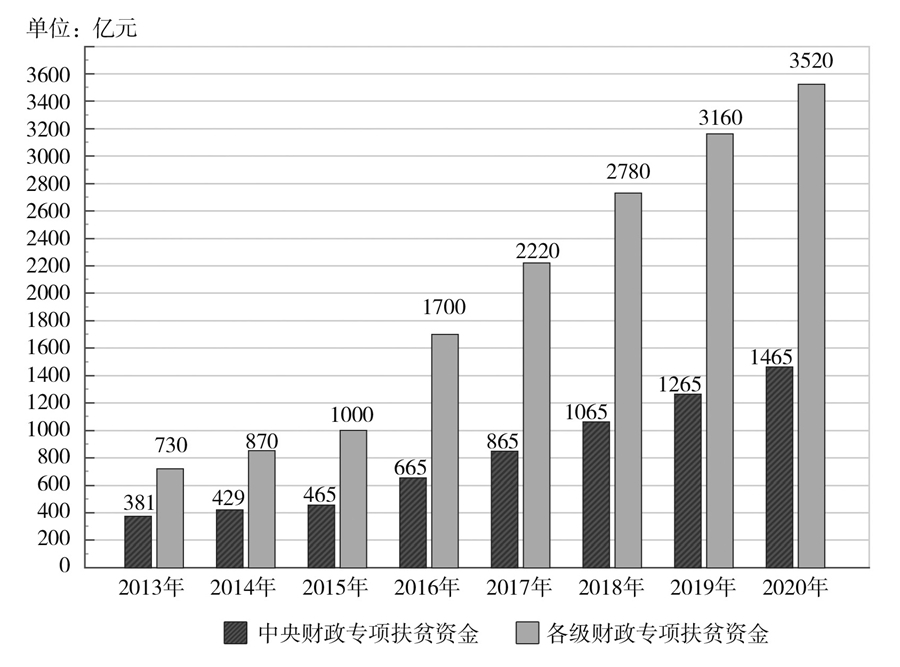
\includegraphics{fig/4.jpg}
    \caption{脱贫攻坚以来财政专项扶贫资金投入情况}
    \label{fig-4}
\end{figure}

\begin{zhuanlan}[脱贫攻坚资金投入]
    脱贫攻坚以来,中国坚持脱贫攻坚投入力度同打赢脱贫攻坚战要求相匹配,持续加大财政投入。中央、省、市、县财政专项扶贫资金累计投入近1.6万亿元,其中中央财政累计投入6601亿元。土地增减挂指标跨省域调剂和省域内流转资金4400多亿元。扶贫小额信贷累计发放7100多亿元,扶贫再贷款累计发放6688亿元,金融精准扶贫贷款发放9.2万亿元。东部9省市共向扶贫协作地区投入财政援助和社会帮扶资金1005亿多元,东部地区企业赴扶贫协作地区累计投资1万多亿元。统筹整合使用财政涉农资金,强化扶贫资金监管,确保把钱用到刀刃上。真金白银的投入,为打赢脱贫攻坚战提供了强大资金保障。
    \label{col-12}
\end{zhuanlan}

\subsection{用发展的办法消除贫困}

贫困问题说到底是发展问题。作为拥有14亿人口、世界上最大的发展中国家,发展是解决包括贫困问题在内的中国所有问题的关键。中国共产党始终把发展作为执政兴国的第一要务,集中精力搞建设、谋发展,通过发展解决不平衡不充分问题,创造了经济快速发展奇迹和社会长期稳定奇迹。把改革作为消除贫困的重要推动力,从新中国成立后进行土地改革、建立社会主义制度,到改革开放后实行家庭联产承包责任制,到确立社会主义市场经济体制、全面免除农业税,再到中共十八大以来实行农村承包地所有权、承包权、经营权“三权分置”和推进农村集体产权制度改革,不断消除导致贫困的制度性、结构性因素,不断促进农村发展、农民增收。积极顺应全球化潮流,坚定不移扩大对外开放,对外贸易持续快速增长,为广大农村劳动力创造了大量就业岗位、拓宽了增收渠道。新中国成立以来特别是改革开放以来,中国经济社会快速发展,经济总量不断跃升,综合实力显著提升,既对减贫形成了强大的带动效应,也为大规模扶贫开发奠定了坚实基础、提供了有力保障。

中国减贫实践表明,发展是消除贫困最有效的办法、创造幸福生活最稳定的途径。唯有发展,才能为经济社会发展和民生改善提供科学路径和持久动力;唯有发展,才能更好保障人民的基本权利;唯有发展,才能不断满足人民对美好生活的热切向往。

\subsection{立足实际推进减贫进程}

贫困问题具有多样性和复杂性,致贫原因也呈现差异性和多元性。中国立足本国国情,根据不同发展阶段和经济社会发展水平,根据贫困人口规模、分布、结构等的变化,科学制定减贫标准、目标、方略,不断创新减贫理念、方法、手段,循序渐进、持续用力、滴水穿石。新中国成立后,主要是通过社会制度变革和大规模社会主义建设减缓贫困。改革开放以来,主要是通过农村经济体制改革和经济增长带动减贫,重点采取开发式扶贫方针,引导贫困地区和贫困群众以市场为导向,调整经济结构,开发当地资源,发展商品生产,提高自我积累、自我发展能力。进入新时代,在继续坚持开发式扶贫的同时,实施精准扶贫方略,扶贫路径由“大水漫灌”转为“精准滴灌”,资源使用方式由多头分散转为统筹集中,扶贫模式由偏重“输血”转为注重“造血”,考评体系由侧重考核地区生产总值转为主要考核脱贫成效。中国根据经济社会发展和减贫事业推进的实际,逐步调整提高扶贫标准,让发展成果更多更好惠及人民群众。

中国减贫实践表明,贫困的发生演变有其自身特点和规律,贫困治理必须从实际出发,科学研判制约减贫和发展的瓶颈因素,找准释放减贫动力的突破口,因时因势因地制宜,不断调整创新减贫的策略方略和政策工具,提高贫困治理效能。

\subsection{发挥贫困群众主体作用}

贫困群众是脱贫致富的主体。扶贫减贫既要借助外力,更要激发内力,才能形成合力。中国充分尊重、积极发挥贫困群众主体作用,激发培育贫困群众内生动力,增强参与发展、共享发展、自主发展的能力,使贫困群众不仅成为减贫的受益者,也成为发展的贡献者。坚持扶贫与扶志扶智相结合,既富口袋,更富脑袋,让贫困群众既有脱贫致富的想法,又有脱贫致富的办法。依托农民夜校、新时代讲习所等,加强教育培训,提升贫困群众发展生产和务工经商的基本技能。改进扶贫方式,建立正向激励、比学赶超的有效机制,更多采用生产奖补、劳务补助、以工代赈等方式,激励贫困群众依靠劳动创造幸福。大力宣传自强不息、奋斗脱贫的先进典型,广泛开展生动活泼、形式多样的宣传教育,引导贫困群众树立“宁愿苦干、不愿苦熬”的观念,用双手改变贫困落后面貌。

中国减贫实践表明,人民是历史的创造者、推动者,是顶天立地的真正英雄。只要坚持为了人民、依靠人民,尊重人民主体地位和首创精神,激励贫困群众自力更生、艰苦奋斗的内生动力,就一定能够战胜贫困。

\subsection{汇聚各方力量形成强大合力}

扶贫减贫是艰巨复杂的系统工程,需要调动各方积极参与。为打赢脱贫攻坚战,中国共产党依托严密组织体系和高效运行机制,广泛有效动员和凝聚各方力量,构建政府、社会、市场协同推进,专项扶贫、行业扶贫、社会扶贫互为补充的大扶贫格局,形成跨地区、跨部门、跨单位、全社会共同参与的多元主体的社会扶贫体系。加强东西部扶贫协作和对口支援(专栏\ref{col-13}),推动省市县各层面帮扶,促进人才、资金、技术向贫困地区流动,实现优势互补,缩小区域差距。积极开展定点扶贫,组织各级党政机关、人民团体、国有企事业单位和军队帮扶贫困县或贫困村(专栏\ref{col-14})。各民主党派、工商联和无党派人士充分发挥各自优势,为打赢脱贫攻坚战献智献力。积极推动各行各业发挥专业优势,开展产业扶贫、科技扶贫、教育扶贫、文化扶贫、健康扶贫、消费扶贫。广泛动员民营企业参与扶贫开发,引导市场开发能力强的主体进入资源开发潜力大的地区,实现互惠互利、共同发展(专栏\ref{col-15})。广泛动员社会组织、公民个人积极参与脱贫攻坚,开展扶贫公益活动。设立国家扶贫日,建立脱贫攻坚国家荣誉制度,表彰脱贫攻坚先进典型,营造了人人愿为、人人可为、人人能为的社会帮扶氛围。

中国减贫实践表明,只有动员和凝聚各方力量,引导全社会关爱贫困群众、关心减贫事业、投身脱贫行动,形成共同意志、共同行动,聚力攻坚克难,才能最终战胜贫困顽疾。

\begin{zhuanlan}[东西部扶贫协作和对口支援]
    东西部扶贫协作和对口支援是实现先富帮有后富、最终实现共同富裕目标的重大举措。东部9个省份结对帮扶中西部14个省份,东部343个经济较发达县(市、区)与中西部573个贫困县开展“携手奔小康”行动。2015年至2020年,东部9个省份共向扶贫协作地区投入财政援助资金和社会帮扶资金1005亿多元,互派干部和技术人员13.1万人次,超过2.2万家东部企业赴扶贫协作地区累计投资1.1万亿元。东部省份和部分中央单位开展对口支援西藏自治区、新疆维吾尔自治区、青海省,组织实施全国教育、医疗人才“组团式”援藏援疆,选派优秀教师、医生开展组团支援,从中央单位选派干部到西部地区、老工业基地、革命老区挂职。
    \label{col-13}
\end{zhuanlan}

\begin{zhuanlan}[中央单位定点扶贫和军队扶贫]
    中央单位通过政策倾斜、资金投入、项目引进、智力支持、科技支撑等方式,开展定点扶贫。脱贫攻坚以来,共有307家中央单位定点帮扶592个国家扶贫开发工作重点县;2013年至2020年,中央单位累计投入帮扶资金和物资427.6亿元,帮助引进各类资金1066.4亿元,培训基层干部各类技术人才368.8万人次。军队帮扶4100个贫困村,92.4万贫困群众实现脱贫。
    \label{col-14}
\end{zhuanlan}

\begin{zhuanlan}[“万企帮万村”精准扶贫行动]
    “万企帮万村”精准扶贫行动是以民营企业为帮扶方,以贫困村、贫困户为帮扶对象,以产业、就业、公益、智力扶贫为主要帮扶形式,帮助贫困村加快脱贫进程。2015年至2020年底,累计组织动员12.7万家民营企业参与"万企帮万村”精准扶贫行动,精准帮扶13.91万个村(其中贫困村7.32万个),共带动和惠及1803.85万贫困人口。
    \label{col-15}
\end{zhuanlan}

中国特色减贫道路,是中国人民在中国共产党的领导下,经过长期艰辛探索开创出来的一条成功道路。中国消除绝对贫困的成功实践和宝贵经验,深化了对人类减贫规律的认识,丰富发展了人类反贫困理论,提振了各国特别是广大发展中国家消除绝对贫困的信心,为其他国家选择适合自己的减贫发展道路提供了参考和借鉴,为破解现代国家治理难题、开辟人类社会发展更加光明的前景提供了中国方案。

\section{携手共建没有贫困共同发展的人类命运共同体}

世界好,中国才能好;中国好,世界才更好。中国始终把自身命运与世界各国人民命运紧密相连,在致力于消除自身贫困的同时,积极参与国际减贫合作,做国际减贫事业的倡导者、推动者和贡献者,与各国携手共建没有贫困、共同发展的人类命运共同体。

\subsection{中国的减贫和发展加快全球减贫进程}

100年来,在中国共产党领导下,中国人民从翻身解放到解决温饱、从基本小康到全面小康,中国以自己的发展为人类反贫困作出重大贡献。改革开放以来,按照现行贫困标准计算,中国7.7亿农村贫困人口摆脱贫困;按照世界银行国际贫困标准,中国减贫人口占同期全球减贫人口70\%以上。在全球贫困状况依然严峻、一些国家贫富分化加剧的背景下,中国打赢脱贫攻坚战,提前10年实现《联合国2030年可持续发展议程》减贫目标,显著缩小了世界贫困人口的版图,“为实现2030年可持续发展议程所描绘的更加美好和繁荣的世界作出了重要贡献”\endnote{2021年2月,中国宣布消除绝对贫困。联合国秘书长古特雷斯致信习近平主席,表示“这一重大成就为实现2030年可持续发展议程所描绘的更加美好和繁荣的世界作出了重要贡献”,“中国取得的非凡成就为整个国际社会带来了希望,提供了激励”。}。作为世界上最大的发展中国家,中国实现了快速发展与大规模减贫同步、经济转型与消除绝对贫困同步,如期全面完成脱贫攻坚目标任务,大大加快了全球减贫进程,谱写了人类反贫困历史新篇章。

\subsection{国际社会对中国减贫提供支持和援助}

新中国成立后,努力打破外部封锁,积极开展对外交流合作,争取国际社会支持。改革开放以来,中国与联合国发展系统和世界银行在扶贫领域开展广泛合作,同时接受部分发达国家提供的援助、实施减贫合作项目,不仅在资金投入、知识转移、技术援助等方面获得支持,而且学习借鉴国际社会先进的扶贫理念与方式方法,推动了中国减贫事业发展。中国先后与联合国开发计划署、世界银行等国际机构和组织合作,在部分贫困县实施外资扶贫项目,引进各种优惠贷款和无偿援助。国际减贫交流合作项目缓解了项目区贫困人口的贫困程度,推动了中国减贫的制度创新和管理水平提升,为项目区的可持续发展奠定了基础。对国际社会给予的宝贵支持和帮助,中国人民永远铭记在心。中华民族是懂得感恩、投桃报李的民族,中国始终在力所能及的范围内为其他国家减贫和发展提供支持。

\subsection{中国积极开展国际减贫交流合作}

中国积极参与全球贫困治理,不断深化减贫领域交流合作,推动建立以相互尊重、合作共赢为核心的新型国际减贫交流合作关系,携手增进各国人民福祉。

支持广大发展中国家减贫发展。新中国成立伊始,在国家百废待兴、财力紧张的情况下,即向有关国家提供援助,为发展中国家争取民族独立和解放、促进经济社会发展提供了支持。改革开放后,中国对外援助内容更加丰富、形式更加多样,促进了中国与其他发展中国家的共同发展。进入新时代,中国担负大国责任,推动对外援助向国际发展合作转型升级,为破解全球发展难题、落实联合国2030年可持续发展议程提出中国方案、贡献中国智慧、注入中国力量。习近平主席在多个国际重大场合宣布中国开展国际发展合作的一系列务实举措,已按期落实或正在按照进度有序推进(专栏\ref{col-16})。中国发起共建“一带一路”倡议,推动更大范围、更高水平、更深层次的区域经济社会发展合作,支持帮助相关国家更好实现减贫发展。据世界银行研究报告,共建“一带一路”将使相关国家760万人摆脱极端贫困、3200万人摆脱中度贫困。新中国成立70多年来,中国向亚洲、非洲、拉丁美洲和加勒比地区、大洋洲和欧洲等地区160多个国家和国际组织提供多种形式的援助,减免有关国家债务,为广大发展中国家落实千年发展目标提供帮助。

\begin{zhuanlan}[习近平主席宣布一系列国际发展合作重大项目]
    中国开展国际发展合作,既有庄重的承诺,也有实实在在的举措。习近平主席在多个国际场合宣布一系列国际发展合作重大项目。

    2015年联合国成立70周年系列峰会期间,习近平主席宣布5年内向发展中国家提供“6个100”项目支持(包括100个减贫项目、100个农业合作项目、100个促贸援助项目、100个生态保护和应对气候变化项目、100所医院和诊所、100所学校和职业培训中心),帮助实施100个“妇幼健康工程" 和100个“快乐校园工程”,设立南南合作援助基金,设立中国-联合国和平与发展基金,提供来华培训和奖学金名额,免除有关国家无息贷款债务,设立南南合作与发展学院和国际发展知识中心等重要举措。

    在2015年中非合作论坛约翰内斯堡峰会上,习近平主席宣布3年内,同非方重点实施中非工业化,农业现代化基础设施金融、绿色发展、贸易和投资便利化、减贫惠民、公共卫生、人文、和平与安全等“十大合作计划”,中国承诺提供600亿美元资金支持。

    在2017年首届“一带一路"国际合作高峰论坛上,习近平主席宣布未来3年内向参与"一带一路"建设的发展中国家和国际组织提供600亿元人民币援助,建设更多民生项目;向沿线发展中国家提供20亿元人民币紧急粮食援助,向南南合作援助基金增资10亿美元,在沿线国家实施100个“幸福家园”、100个“爱心助困”、100个“康复助医"等项目;向有关国际组织提供10亿美元等一系列重要举措。

    在2018年中非合作论坛北京峰会上,习近平主席宣布未来3年和今后一段时间重点实施产业促进、设施联通、贸易便利、绿色发展、能力建设、健康卫生、人文交流、和平安全等“八大行动”。为推动行动顺利实施,中国愿以政府援助、金融机构和企业投融资等方式,向非洲提供600亿美元支持。

    在2019年第二届“一带一路”国际合作高峰论坛上,习近平主席宣布实施“一带一路”应对气候变化南南合作计划,深化农业、卫生、减灾、水资源等领域合作,邀请1万名代表来华交流,鼓励和支持沿线国家社会组织广泛开展民生合作,持续实施“丝绸之路”中国政府奖学金项目等一系列重要举措。

    在2020年第73届世界卫生大会视频会议开幕式上,习近平主席宣布两年内提供20亿美元国际援助,与联合国合作在华设立全球人道主义应急仓库和枢纽,建立30个中非对口医院合作机制、中国新冠疫苗研发完成并投入使用后将作为全球公共产品、同二十国集团成员一道落实“暂缓最贫困国家债务偿付倡议”等中国支持全球抗疫的一系列重大举措。
    \label{col-16}
\end{zhuanlan}

实施惠及民生的国际减贫合作项目。在亚洲地区,中国与东盟国家共同开展乡村减贫推进计划,在老挝、柬埔寨、缅甸三国乡村基层社区实施“东亚减贫示范合作技术援助项目”(专栏\ref{col-17})。在非洲地区,中国为非洲国家援建水利基础设施、职业技术学校、社会保障住房等设施,打造农业合作示范区,推进实施中非菌草技术合作、中非友好医院建设、非洲疾控中心总部建设等项目(专栏\ref{col-18})。在南太平洋地区,中国推动落实对太平洋岛国无偿援助、优惠贷款等举措,开展基础设施建设和农业、医疗等技术合作援助项目。在拉美地区,援建农业技术示范中心,帮助受援国当地民众摆脱贫困。中国还与联合国教科文组织合作设立国际农村教育研究与培训中心等机构,面向非洲、东南亚等国家实施农村教育转型、教师培训等项目。

\begin{zhuanlan}[东亚减贫示范合作技术援助项目]
    2014年11月,中国提出实施“东亚减贫合作倡议”,开展乡村减贫推进计划,建立东亚减贫合作示范点。自2017年7月起,中国在老挝、柬埔寨、缅甸等国6个贫困村实施“东亚减贫示范合作技术援助项目”,为示范村新建了饮水桥梁、道路、电力等基础设施,建设了村民活动中心、卫生室、学校等公共服务设施,为贫困户新建和改建了住房、厕所和环保设施,改善了示范村的生产生活条件和村容村貌。组织村民开展肉牛和家禽等养殖、玉米和蔬菜等种植、水稻和花生等作物良种良法示范、织布和竹编等手工业、乡村旅游、庭院经济、外出务工、技术培训等,多渠道增加村民收入,提升了示范村和村民的自我发展能力。“东亚减贫示范合作技术援助项目”的模式及成效受到东盟国家部长、联合国粮农组织等国际机构代表的高度评价,称其为“减贫合作的标杆”。
    \label{col-17}
\end{zhuanlan}

\begin{zhuanlan}[中国对非农业技术援助村级示范项目]
    从2011年起,中国国际扶贫中心在坦桑尼亚莫罗戈罗省佩雅佩雅村推广中国玉米种植技术,这是中国第一个在村级层面开展的对非援助项目。项目旨在把通过培育小农户生产能力提高农业生产效率、进而改善粮食安全和缓解贫困的中国经验应用到坦桑尼亚减贫实践中。中国农业专家走进田间地头,手把手向当地村民传授农耕技术,改变了当地粗放播种的耕作模式,玉米平均增产2-3倍。农民吃饭问题明显改善,同时还有余粮出售增加收入,一定程度上缓解了贫困。当地农户将中国专家带来的玉米种植技术亲切地称为“中国技术”。2018年,莫罗戈罗省进一步扩大中国玉米种植技术推广范围,发起“千户万亩玉米增产示范工程”。
    \label{col-18}
\end{zhuanlan}

分享交流减贫经验。通过搭建平台、组织培训、智库交流等多种形式,开展减贫交流,分享减贫经验。在国际消除贫困日,中国与联合国驻华机构联合举办减贫与发展高层论坛活动。中国发起中国-东盟社会发展与减贫论坛、人类减贫经验国际论坛,举办中非减贫与发展会议、“摆脱贫困与政党的责任”国际理论研讨会、改革开放与中国扶贫国际论坛等一系列研讨交流活动。与东盟秘书处和东盟有关国家合作,面向基层村官(社区官员)实施“东盟+中日韩村官交流项目”。与有关国家和地区组织合作开展国际减贫培训,2012年以来,共举办130余期国际减贫培训班,来自116个国家(组织)的官员参加培训。

当今世界正处于百年未有之大变局,新冠肺炎疫情仍在全球蔓延,贫穷、饥饿、疾病侵蚀着人们追求美好生活的希望和信心。建设什么样的世界、人类文明走向何方,攸关每个国家、每个人的前途和命运。每个人都有过上好日子的权利。各国应担负起对人民的责任,积极推进减贫发展,让公平正义的阳光冲破贫困落后的阴霾,照亮繁荣发展的美好未来。中国愿同各国加强减贫交流合作,携手推进国际减贫进程,为构建没有贫困、共同发展的人类命运共同体作出更大贡献。

\sect{结束语}

中国打赢脱贫攻坚战,如期实现脱贫攻坚目标任务,中国人民在创造美好生活、实现共同富裕的道路上迈出了坚实的一大步。同时,中国仍是世界上最大的发展中国家,仍面临人民日益增长的美好生活需要和不平衡不充分的发展之间的矛盾。解决发展不平衡不充分问题、缩小城乡区域发展差距、实现人的全面发展和全体人民共同富裕,仍然任重道远。

脱贫摘帽不是终点,而是新生活、新奋斗的起点。中国共产党将始终坚守为人民谋幸福、为民族谋复兴的初心和使命,始终把人民放在最高位置,为实现人的全面发展和全体人民共同富裕驰而不息、接续奋斗,不断增进人民福祉,更好满足人民对美好生活的新期待,让全体人民过上好日子。

民族要复兴,乡村必振兴。打赢脱贫攻坚战之后,中国将持续巩固拓展脱贫攻坚成果,做好同乡村振兴有效衔接,实现“三农”工作重心的历史性转移。中国将立足新发展阶段、贯彻新发展理念、构建新发展格局,把解决好“三农”问题作为重中之重,坚持农业农村优先发展,走中国特色社会主义乡村振兴道路,以更有力的举措、汇聚更强大的力量全面推进乡村振兴。

到2035年,中国将基本实现社会主义现代化,乡村振兴取得决定性进展,农业农村现代化基本实现。那时的中国乡村,农业结构得到根本性改善,农民就业质量显著提高,相对贫困进一步缓解,共同富裕迈出坚实步伐;城乡基本公共服务均等化基本实现,城乡融合发展体制机制更加完善;乡风文明达到新高度,乡村治理体系更加完善;农村生态环境根本好转,美丽宜居乡村基本实现。

到2050年,中国将全面建成社会主义现代化强国,实现第二个百年奋斗目标,乡村全面振兴。那时的中国乡村,农业强、农村美、农民富,经济社会全面进步,各项事业繁荣发展。那时的中国,全体人民共同富裕基本实现,中国人民享有更加幸福安康的生活,中国向着实现人的全面发展和全体人民共同富裕更高目标继续迈进。

中国的发展离不开世界,世界的发展也离不开中国。中国始终将自身发展与人类发展紧密相连,始终做世界和平的建设者、全球发展的贡献者、国际秩序的维护者。繁荣发展的未来中国,是更加开放包容的中国,是与世界形成更加良性互动的中国,是为建设更加美好的世界作出更大贡献的中国。

\sect{附录:中国扶贫标准的变化和调整}

根据国民经济社会发展水平和贫困人口基本生活需求确定扶贫标准,是中国实施大规模、有计划、有组织扶贫以来一直的做法。

中国第一次制定扶贫标准是1986年,为206元,对应的贫困人口数量为1.25亿,主要解决温饱问题。2001年制定第一个十年农村扶贫开发纲要时,将扶贫标准提高到865元,对应的贫困人口数量为9422.8万。2011年制定第二个十年农村扶贫开发纲要时,将扶贫标准提高到2300元(2010年不变价),对应的贫困人口数量为1.22亿。

脱贫攻坚以来,中国的贫困人口识别和退出以户为单位,主要衡量标准是“一收入”“两不愁三保障”。“一收入”就是该户年人均纯收入稳定超过现行国家扶贫标准,“两不愁三保障”就是稳定实现不愁吃、不愁穿和义务教育、基本医疗、住房安全有保障。中国的贫困人口退出标准是综合性多维标准,不仅衡量收入水平,还考量贫困人口生存权发展权的实现程度,体现了中国经济社会发展实际和全面建成小康社会的基本要求。

\theendnotes

\end{document}
